\chapter{Antonia Maury, Aydte.}
\label{cap:antonia}

\lettrine[lines=2]{C}{uando Cecilia} entró en la oficina de Antonia la
encontró sentada frente a la computadora. En sus manos se veía, ahora
con claridad al encontrarse más cerca y sin ser deslumbrada por la luz
del Sol, el objeto semicilíndrico con el que seguramente creó las
manchas que tanto la alarmaron en el jardín. Tendría unos 20
centímetros de longitud y un diámetro de aproximadamente 5
centímetros. Presentaba curiosos agujeros o ranuras, dispuestos en lo
que parecía una especie de azar controlado por una ley secreta.

---Como recordarás, hace unos días la familia Ciaffone Hallak,
patrocinante de esta benemérita institución, donó una impresora 3D a
Harvard ---rememoró Antonia con voz clara---.  \director{} quería que
diseñara unos posavasos para la sala de reuniones ---Antonia subrayó
esta última palabra con la voz y con el gesto, y Cecilia no pudo
reprimir una risita cómplice recordando un suceso no muy
lejano---. Pero a mí se me ocurrió algo más... interesante.

\begin{figure}[t]
  \centering
  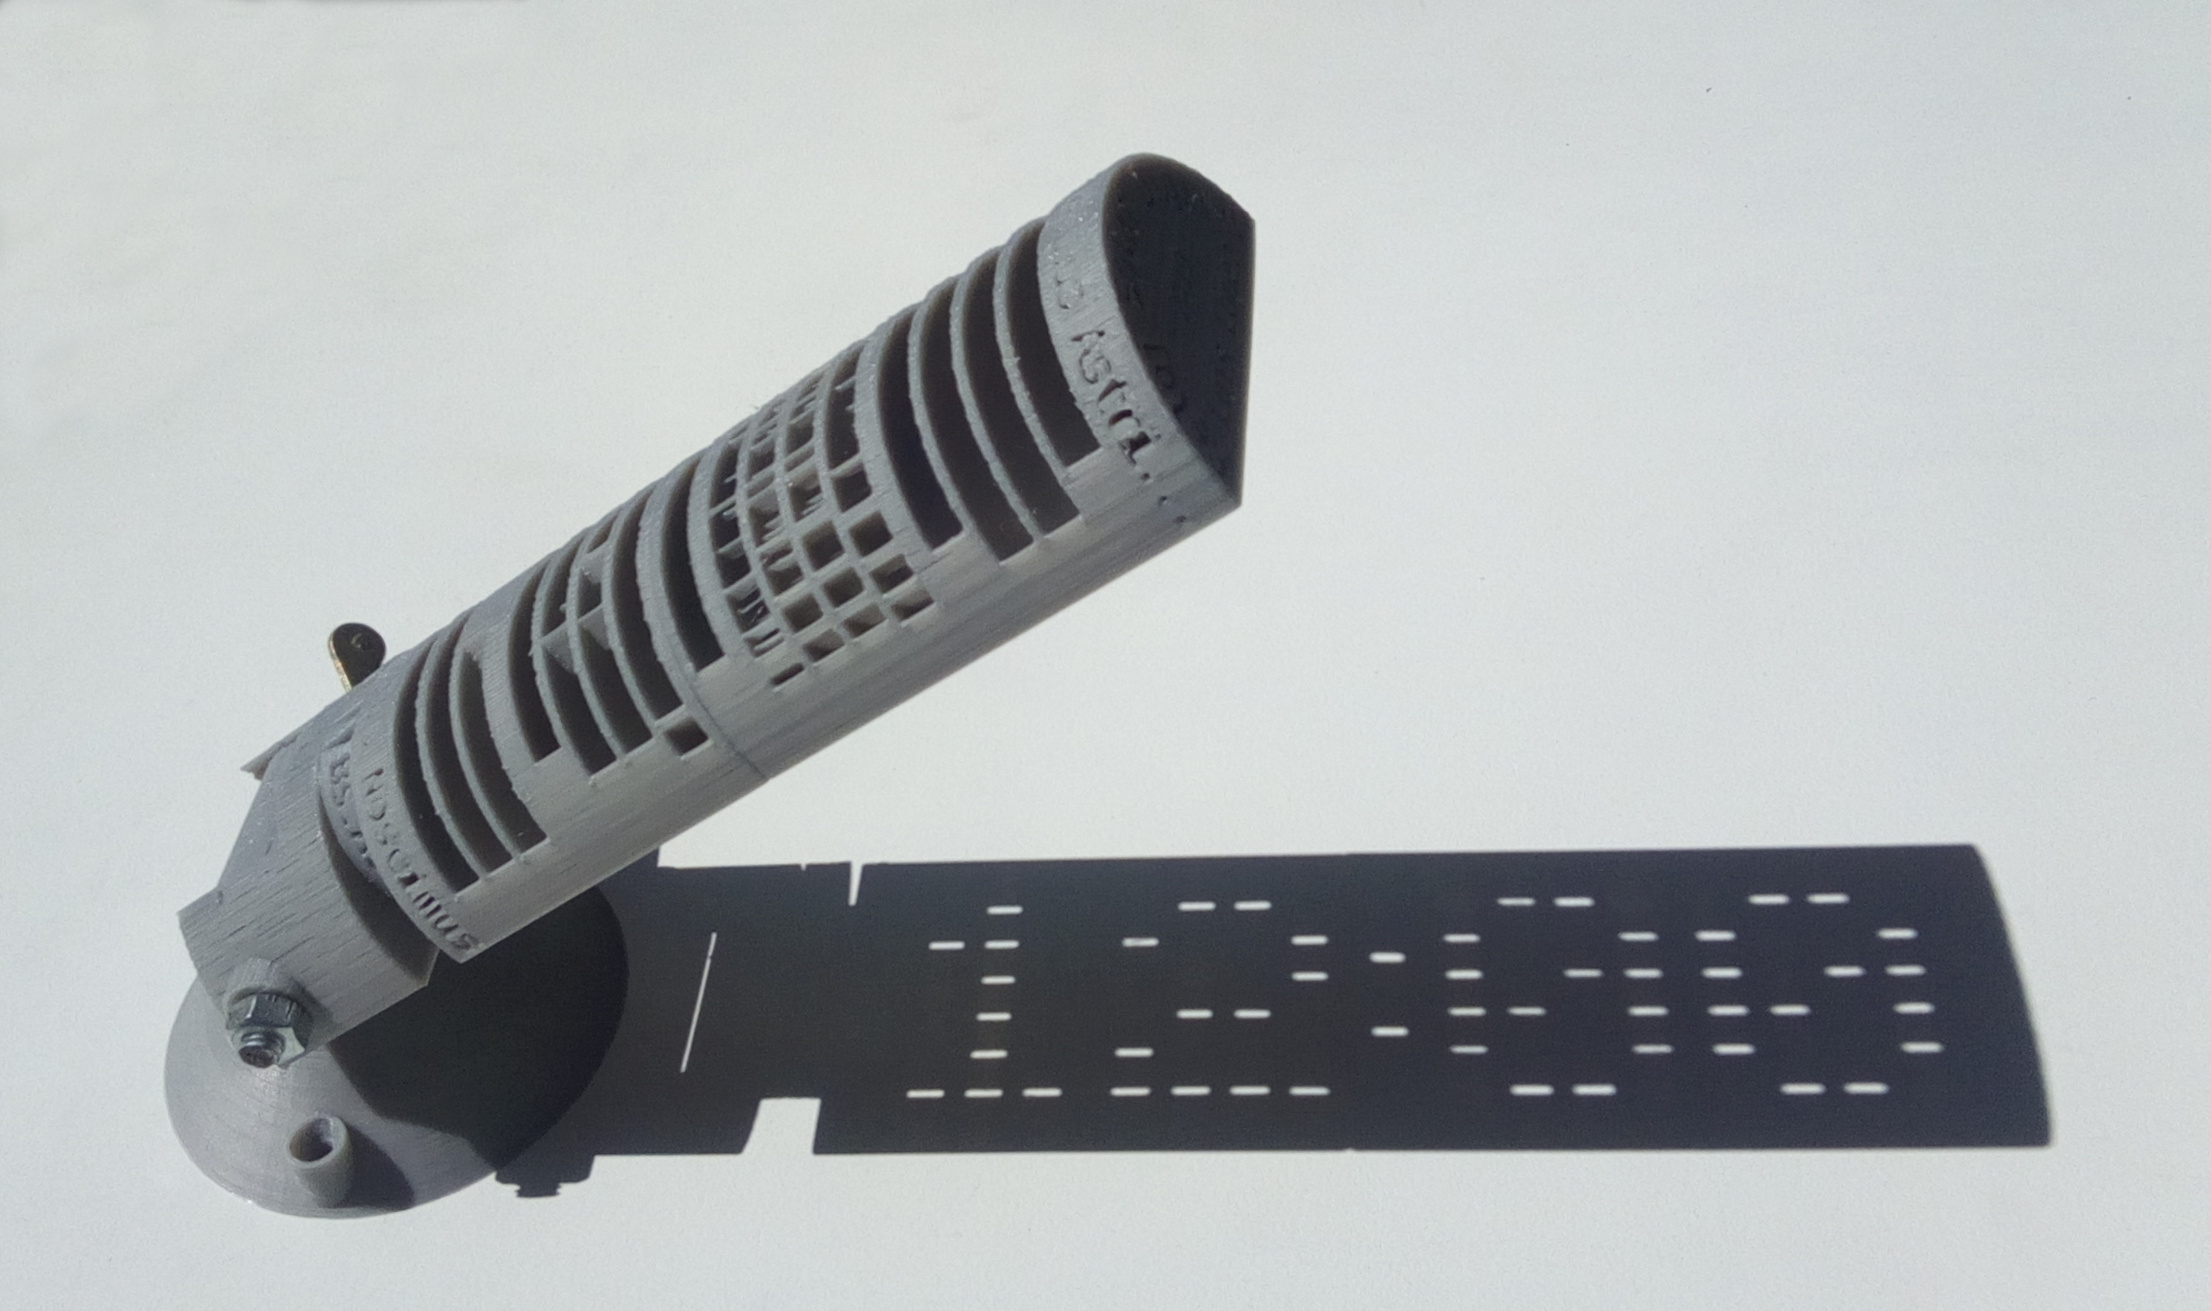
\includegraphics[width=\textwidth]{imagenes/reloj-equinoccio}
  \caption{El mágico objeto con el que Antonia produjo las manchas que
    alarmaron a Cecilia, y que pronto encenderá su
    entusiasmo.}%\iftoggle{libro}{\vspace{128in}}{}
  \label{fig:reloj-equinoccio}
\end{figure}

Cecilia sonreía con delicada ternura mientras escuchaba y miraba a
Antonia. Antonia se mantenía siempre igual: periférica, brusca,
irritable, indiferente, vulnerable. Siempre en guerra con \director{}
y ansiosa por compartir sus resultados ---de los cuales era la primera
en aburrirse y dejar de la\-do--- con sus compañeras, sin importarle
lo que éstas estuvieran haciendo al momento de interrumpirlas con los
productos de su impredecible pulsión por hacer y deshacer. Cecilia
había descubierto que el tiempo, junto a ella, pasaba mejor.



%%% Local Variables:
%%% mode: latex
%%% TeX-master: "../libro"
%%% End:
